\section{Research Method}
\label{ResearchMethod}
In this study, the researchers combine the application of RFID and OTP (One-Time Password) authentication algorithm to achieve reliable Multi-Factor Authentication (MFA) method technique.

\subsection{Multi-Factor Authentication}
Multi-factor authentication (MFA) is a security approach for using more than one authentication tool from the available independent credentials to verify users. Multi-factor authentication combines two or more layers of the Authentication program: what users know (keywords), what users have (security tokens) and (biometric verification) \cite{oke2017developing}. The purpose of the MFA is to create layered defences and make it more difficult for unauthorised people to access targets such as physical locations, computing devices, networks or databases. If one factor is compromised or damaged, the attacker still has at least one more barrier to be broken before successfully breaking the target. This is widely known as the most secure method for authenticating access to data or applications \cite{shah2015multi}.
\subsection{One-Time Password}
One-Time Password (OTP) is an automatically generated numeric or alphanumeric string that authenticates a user for a single transaction or session \cite{huang2013rfid}. OTP is more secure than a fixed password, especially user-generated passwords, which may be vulnerable to attack after a period. OTPs may override authentication login information or may use in addition to adding other security layers. OTP can be synchronised or based on mathematical algorithms, OTPs synchronise to a more well-known type. For time synchronised OTPs, tokens are usually pocket-sized fobs with small screens displaying numbers. The number changes every time depending on the configuration of the token \cite{jacob2015mobile}.
\subsection{Authentication Process}
The Authentication process in the application of the entire authentication system divides into two parts namely part (IN) and (OUT):

\subsubsection{IN Process} 
In the process (IN) consists of 4 steps, namely:

\begin{enumerate}
    \item 
    User Login Account to local system via a smartphone device.
    \item
     User tapping RFID card to attend
    \item 
    Verify the data card and generate the OTP
    \item
    Generate the OTP code then send it to the user's account.
\end{enumerate}
\begin{figure}[ht]
\begin{center}
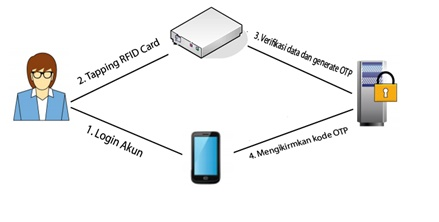
\includegraphics[width=8cm]{figures/Masuk.jpg}
\end{center}
\caption{(IN) Process.
\label{eq:30}}
\end{figure}  

\subsubsection{OUT Process} 
In the process (OUT) consists of 4 steps, namely:

\begin{enumerate}
    \item 
    User Login Account to local system via a smartphone device.
    \item
     User tapping RFID card
    \item 
    User Entering the existing OTP code and the system will verify the RFID ID and the inputted OTP code.
    \item
    If appropriate, Data Successfully saved.
\end{enumerate}
\begin{figure}[ht]
\begin{center}
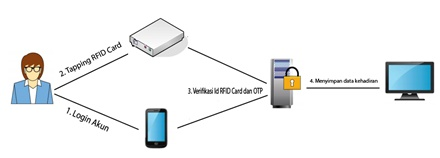
\includegraphics[width=8cm]{figures/Keluar.jpg}
\end{center}
\caption{(OUT) Process.
\label{eq:30}}
\end{figure} 